
% Background Chapter
%%%
% New organisation:
%
% Introduction and Literature Review
%   Tropospheric ozone and air quality . . . . .
%   Isoprene and other VOCs . . . . . . . . . . .
%   Formaldehyde (HCHO) . . . . . . . . . . . .
%   Models . . . . . . . . . . . . . . . . . . . . .
%   Aims?
%%%%%%
\chapter{Introduction and Literature Review} % Chapter Title
\label{LR}
  
\section{Tropospheric ozone and air quality}
  \label{LR:O3andAQ}
  \subsection{Air Quality}
    \label{LR:O3andAQ:AQ}
    %%% AUSTRALIA
    
    % Moved to intro    
    
    \subsubsection{Ozone}
      %%% OZONE
      
      
      
    
    \subsubsection{Particulate matter and SOA}
      
    
    
    \subsubsection{Factors influencing ozone and PM}
      %\label{LR:O3andAQ:AQfactors}
      
    \subsubsection{How do we measure air quality?}
      
      
      
      
      
  \subsection{Ozone transported from the stratosphere}
    
    
    
    
    
    
    
    
  

  \subsection{Ozone formed in the troposphere}
    \label{LR:O3andAQ:BiogenicOzonePrecursors}
    
    
    
\section{Hydroxyl (OH) and other radicals}
  \label{LR:Radicals}
  
  
  
  
  

\section{Isoprene and other VOCs}
  \label{LR:VOCs}
  \subsection{What are VOCs}
    

    
  \subsection{What do they Do?}
    
    
    
  \subsection{Isoprene Cascade}
  
    
  \subsection{How and where do we measure them?}
    

  
  
  \subsection{Emissions estimates}
    \label{LR:VOCs:EmissionsEstimates}
    
    
  
\section{Formaldehyde (HCHO)}
  \label{LR:HCHO}
  
  %Paragraphs moved to Intro
  
  \subsection{How HCHO is measured}
    % how to measure HCHO
    There are a few ways to measure HCHO, including Fourier Transform Infra-Red Spectrometry (FTIR) and Differential Optical Absorption Spectroscopy (DOAS).
    The DOAS technique takes advantage of the optically thin nature of HCHO in order to linearise the radiance differential through air masses with and without HCHO, using the Beer-Lambert intensity law.
    This method works for both in the home HCHO detection and global measurements from in-situ and remote sensing instruments (\cite{Guenther1995, Abad2015, Davenport2015}).
    As a trace gas HCHO interferes with light over a few wavelength bands, which allows instruments to detect concentrations between a known light source and a detector.
    Figure \ref{LR:fig:HCHOSpectrum} shows the interference spectrum of HCHO as well as a typical band used to examine interference in the DOAS technique.
    One difficulty is that this interference is relatively small (HCHO is optically thin) and other compounds absorb light at similar wavelengths (\cite{Davenport2015}).
    FTIR measurements can have a range of uncertainties, including systematic and random measurement errors and uncertain apriori shape factors and water profiles (eg: \cite{Franco2015}).
    Multiple axis DOAS (MAX-DOAS) uses DOAS over several open path directions and also examines the infra-red light interference.
    In \cite{Franco2015}, an FTIR spectrometer at Jungfraujoch is compared against both MAX-DOAS and satellite data, with two CTMs; GEOS-Chem and IMAGES v2 used to compare total columns and vertical resolution of each instrument.
    Generally satellites use a DOAS based technique, with chemical transport and radiative transfer models used to transform the non-vertical light path interference into vertical column amounts.
    
    \begin{figure}
      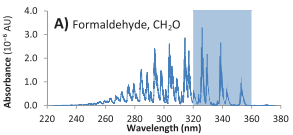
\includegraphics{Figures/HCHO/HCHOAbsorbanceDavenport.png}
      \caption{ %
        HCHO spectrum, with a typical band of wavelengths used for DOAS path measurements.
        This is a portion of an image from \cite{Davenport2015}.}
      \label{LR:fig:HCHOSpectrum}
    \end{figure}
    
    MAX-DOAS is a remote sensing technique which uses several DOAS measurements over different viewing paths.
    In these retrievals, the measurements of light absorption are performed over several elevations in order to add some vertical resolution to the measurement of trace gas concentrations.
    An example of this is shown in figure \ref{LR:HCHO:fig_MAXDOASExample}, which was taken from \cite{Lee2015}.
    Recently MAX-DOAS has been used to examine HCHO profiles in the clean free troposphere (\cite{Franco2015, Schreier2016}) as well as in polluted city air (\cite{Lee2015}).
    Depending on orography and atmospheric composition (ie. the influence of interfering chemicals), MAX-DOAS can be used to split the tropospheric column into two partial columns; giving a small amount of vertical resolution to HCHO measurements \citep[eg.]{Franco2015, Lee2015}.
    
    \begin{figure}
      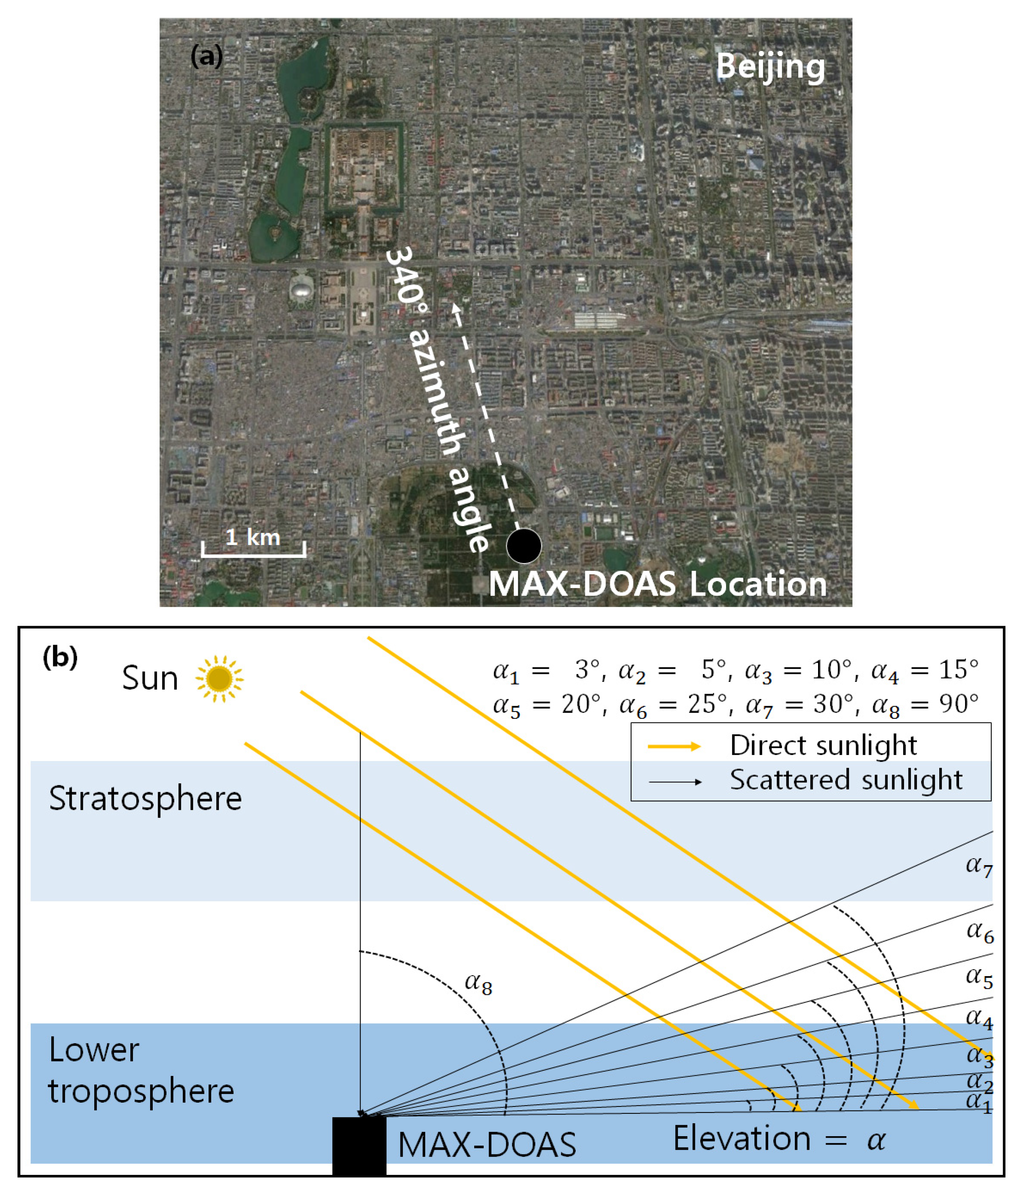
\includegraphics[width=\textwidth]{Figures/MAXDoasExample.png}
      \caption{ Image from \cite{Lee2015}.}
      \label{LR:HCHO:fig_MAXDOASExample}
    \end{figure}
    
    DOAS methods are based on light interference and absorption through air masses.
    Other types of measurement involve directly measuring the air, and determining chemical compounds through their physical properties.
    A proton transfer reaction mass spectrometer (PTR-MS) can be used to determine gas phase evolution of terpene oxidation products (\cite[eg.]{Lee2006a,Nguyen2014,Wolfe2016}).
    This is done through analysis of mass to charge ratios ($m/z$) of ionised air masses which are then identified as chemical compounds.
    \cite{Nguyen2014} use and compare several instruments (including one which is PTR-MS based) in the analysis of isoprene and monoterpene products.
    A Gas Chromatography mass spectrometer (GC-MS) is also able to identify isoprene, monoterpenes, and their products \cite[eg.]{Nguyen2014}.
    % TODO: Explain and find a couple of chamber studies to cite (should already be in my thing)
    
    Other measurement techniques include chromatographic and fluorimetric methods, both of which differ widely from each other and the spectroscopic methods (\cite{Hak2005}).
    \cite{Hak2005} examine a single air mass with 8 instruments using the four techniques (MAX-DOAS, FTIR, chromatographic, and flourimetric), and show that reasonable agreements can be achieved.
    Generally the measurements were somewhat close, the five Hantzsch instruments agreeing to within 11\% (after removing two potentially faulty measurements), although different calibration standards were used.
    Titration for the different calibration solutions could not be resolved, which may account for absolute offsets up to 30\%.
    These differences and non-uniformities between measurements (even among identical instruments) are part of the reason HCHO does not have a consistent network for global measurements like those for GHGs or Ozone (\cite{FortemsCheiney2012}).
  
  \subsection{Sources and sinks}
    \label{LR:HCHO:Sources}
    In the atmosphere HCHO is primarily produced through the oxidation of methane (CH$_4$) by the hydroxyl radical (OH).
    CH$_4$ concentrations are thought to be well constrained in models, with the ACCMIP comparison showing only $\sim3$\% inter-quartile range (\cite{Young2013}).
    Within the continental boundary layer, the major source of HCHO enhancement is VOC emissions reacting with OH radicals in the presence of NO$_X$ (\cite{Wagner2002, Millet2006, Kefauver2014}).
    There is a complex relationship between VOCs, HO$_X$, and NO$_X$, and with higher levels of NO$_X$ the speed that VOCs are converted into HCHO increases, as does the HCHO concentration (\cite{Wolfe2016}).
    Isoprene is the main VOC precursor of HCHO in the continental boundary layer, except near fires or anthropogenic sources of HCHO and precursors (\cite{Guenther1995, Kefauver2014, Wolfe2016}).
    
    Biomass burning (BB) can be a source of HCHO, and various other pollutants, precursors, and aerosols (\cite{Guenther1995, Andreae2001}).
    Additionally HCHO is emitted into the atmosphere directly through fossil fuel combustion, natural gas flaring, ethanol refining, and agricultural activity (\cite{Wolfe2016}).
    Background levels of HCHO are maintained by methane oxidation, while enhancements to regional and continental HCHO are largely driven by isoprene emissions (\cite{Guenther1995, Palmer2003, Shim2005, Kefauver2014}).
    \cite{Atkinson2000} summarised the background formation of HCHO with the following reaction:
    \begin{equation*} \label{LR:HCHO:Sources:eqn_MethaneBackground}
    OH + CH_4 (+ h\nu) + 2NO + 2O_2 \rightarrow OH + HCHO + H_2O + 2O_3
    \end{equation*}
    which shows that photolysis and oxidation of methane forms HCHO and ozone in a process that regenerates the OH radicals.
    
    Other terpenoids (monoterpenes, sesquiterpenes, etc.) can also produce HCHO, although generally to a lesser extent than isoprene, methane and biomass burning (\cite{Guenther2012}).
    Many of the HCHO yields from terpenoids are estimated through chamber studies which examine the products molecular mass and charge after mixing the compound of choice into a known volume of air (\cite[eg.]{Nguyen2014}).
    These conditions generally don't match those of the real world, where ambient air will have a cocktail of these compounds as well as various reactants.
    \cite{Nguyen2014} state that one of their goals is to recreate ambient atmosphere in their chamber studies with more accuracy, in order to improve interpretations and allow more accurate model parameters.
    An important factor in determining the yield of HCHO and other products from BVOCs is the local concentration of NO$_X$.
    \cite{Travis2016} show how modelled surface ozone is overestimated due to high estimates of  NO$_X$ emissions, which affect oxidative capacity and VOC reactions.
    
    %% HCHO SINKS
    HCHO has two major sinks, one being reactions with OH (oxidation), the other being photolysis: the process of being broken apart by photons (\cite{Crutzen1999, Wagner2002, Levy1972, Kefauver2014}).
    These reactions lead to a daytime lifetime of a few hours (\cite{Atkinson2000, Millet2006}).
    Both these loss processes (photolysis, oxidation) form CO and hydroperoxyl radicals (HO$_2$), and have global significance to radiative forcing and oxidative capacity (\cite{Franco2015}).
    The other notable sinks are wet and dry deposition, although these are not as significant (\cite{Atkinson2000}) (TODO: add more cites here).
    
    % Lead into satellite inversion
    In the past, HCHO levels were underestimated by models, often with large discrepancies, due to the poor understanding of methyl peroxy radical (CH$_3$OO) chemistry (\cite{Wagner2002}).
    Nowadays HCHO concentrations are better understood, however precursor emissions are one of the main unknowns (\cite[eg.]{Emmerson2016,Marvin2017}).
    \cite{Marvin2017} found that discrepancies in modelled HCHO concentrations are primarily due to second and later generation isoprene oxidation chemistry.
    
    Formaldehyde formed in the troposphere is mostly due to VOC (roughly one third each: methane, isoprene, others) oxidation.
    We can model this oxidation process in order to work out how much VOC is present based on the total HCHO.
    This requires among other things an idea of which VOCs are present and their yields of HCHO.
    The technique of determining isoprene emissions from satellite detected HCHO is called satellite inversion.
  
  \subsection{Satellite inversion}
    \label{LR:HCHO:SatelliteInversion}
    
    Satellites recording reflected solar spectra use Differential Optical Absorption Spectroscopy (DOAS) to measure various trace gases in the atmosphere, including formaldehyde. 
    Formaldehyde levels in the continental boundary layer are generally dominated by chemical formation due to VOC (largely isoprene) emissions \citep{Kefauver2014}.
    While satellite measurements can only be used during daytime hours, HCHO lifetimes are sufficiently short that any night-time chemistry will not affect midday observations \citep{Wolfe2016}.
    Satellites can be used to measure the seasonal and interannual variability of HCHO over Australia.
    These records can be compared with modeled estimates of HCHO and used as a proxy to estimate isoprene emissions.
    This has been done in North America \citep{Palmer2003, Millet2006}, South America, Africa, China, Europe \citep{Dufour2009}, and recently globally \citep{FortemsCheiney2012, Bauwens2016}.
    Often these works use two forms of measurement such as satellite and aircraft data combined for validation (\cite{Marais2014}).
    There is less information available from satellite measurements at higher latitudes due to increased errors (\cite{DeSmedt2015}).
    
    Using HCHO to determine emissions of isoprene was initially performed by \cite{Palmer2001, Palmer2003}, who used in-situ summertime HCHO measurements over North America as model validation.
    Isoprene emissions fluxes were derived using the Global Ozone Monitoring Experiment (GOME) satellite instrument.
    Palmer's method improved biogenic isoprene emissions estimates (compared with in-situ measurements) over two available inventories: the U.S. EPA Biogenic Emissions Inventory System (BEIS2) and the Global Emissions Inventory Activity (GEIA).
    This showed an inversion technique which could be used to improve large scale emissions estimates without further expensive measurement campaigns.
    
    Initially studies assumed a simple linear steady-state relationship between HCHO and it's precursors (\cite{Palmer2003, Palmer2006, Millet2006}).
    This allowed a simple calculation of isoprene using the measured HCHO, with estimated reaction rates and yields.
    The methodology for calculating VOCs from HCHO is laid out in \cite{Palmer2003}, and takes into account the expected lifetime and reaction rates of the precursor VOCs and HCHO.
    Assuming HCHO is produced quickly from short-lived intermediates, and the column is at steady state:
    \begin{eqnarray*}
      VOC_i \overset{k_i}{\rightarrow} Y_i HCHO
    \end{eqnarray*}
    Where $Y_i$ is HCHO yield per C atom (a measure of how much HCHO will form per gram of C from a VOC within a system), and $k_i$ is the reaction rate.
    Then assuming a steady state of atmospheric HCHO ($\Omega$ molecules $cm^{-2}$) produced by oxidation of VOCs (VOC$_i$) and no horizontal transport:
    \begin{eqnarray*}
      \Omega = \frac{1}{k_{HCHO}} \sum_{i} Y_i E_i
    \end{eqnarray*}
    Where i indexes a chemical species, $k_{HCHO}$ is the HCHO loss rate due to OH and photolysis, Y$_i$ is the molar HCHO yield from oxidation of i, and $E_i$ is emission fluxes ( C atoms $cm^{-2}s^{-1}$).
    
    Estimates of Y$_i$ can be attained from a model as shown in \cite{Millet2006}.
    This involves a reduced major axis (RMA) correlation calculation between modelled HCHO and isoprene columns, multiplied by their loss rates (to photolysis and oxidation) (as a normalising factor).  
    In high NOx environments where HCHO has a lifetime on the order of 30 minutes, it can be used to map isoprene emissions with spatial resolution from 10-100 kms.
    Horizontal transport 'smears' the HCHO signal so that source location would need to be calculated using windspeeds and loss rates (\cite{Palmer2001,Palmer2003}).
    Smearing is explicitly handled in these studies due to the importance of transport and NO$_X$ on forming robust and accurate estimates.
    Over Australia NO$_X$ levels are generally not high enough to ensure quick HCHO formation and we must take extra care that we can account for the transport or 'smearing' caused by slower HCHO formation, details on this process can be found in Section \ref{BioIsop:Methods:Smearing}.
    
    Another method of correcting isoprene emissions using observed HCHO total column involves a Bayesian inversion.
    \cite{Shim2005} work with GOME HCHO observations and GEOS-Chem, looking at areas with high signal to noise ratio (higher HCHO concentrations).
    They show that the model underestimates isoprene emissions and HCHO concentrations by 14-46\%, with the corrected VOC emissions reducing the model biases to 3-25\%.
    
    The Bayesian inversion is also used in \cite{Curci2010}, where a regional CTM (CHIMERE) simulates HCHO, which is compared against OMI observed HCHO and shown to be regionally biased.
    This bias is expected to be caused by errors in MEGANs isoprene emissions estimations.
    The CHIMERE model is used to derive yields of HCHO from the various local VOCs and these are then used in estimating local emissions.
    The model is run initially with emissions of BVOCs and reactive anthropogenic VOCs (RAVOCs) turned off in order to work out the background (b) values of these compounds.
    The Bayesian inversion is used to correct regionally biased biogenic isoprene emissions by optimising these parameters in order to simulate HCHO closest to the observed HCHO levels.
    \cite{Curci2010} uses CHIMERE as the forward model to determine the relationship between HCHO (y), isorene and reactive anthropogenic VOCs (\textbf{x}), using 
    \begin{equation}
    y=\mathbf{K}x + b + \epsilon
    \end{equation}
    where $\epsilon$ are the (assumed) independent errors in measurements.
    K is the Jacobian matrix determined from CHIMERE representing the sensitivity of y to the state variable x.
    This K matrix is used in conjunction with error covariance in x to determine the Maximum A Posteriori (MAP) solution to calculate the optimal estimate of x ($\hat{x}$).
    
    %TODO
    TODO: Read through this list of sources on the hcho to isop process : taken from Wolfe2015
    Such techniques have informed isoprene emission inventories in North America (Abbot et al., 2003; Millet et al., 2008 (\cite{Palmer2003,Millet2006,Palmer2006})), South America ((\cite{Barkley2013}), 2008), Europe (\cite{Curci2010,Dufour2009}), Africa (\cite{Marais2012}), Asia (Fu et al., 2007; Stavrakou et al., 2014), and globally (Fortems-Cheiney et al., 2012; (\cite{Shim2005}); Stavrakou et al., 2009).
    
    
    More recently, full inversions that better account for transport, source attribution, and chemical schemes have been implemented (\cite{FortemsCheiney2012}).
    TODO: full description of this better inversion technique going through FortemsCheiney2012.
    
    Validation is important due to the various uncertainties in the satellite remote sensing process, with apriori assumptions having the greatest effect on structural uncertainty between measurements techniques \cite{Lorente2017}.
    \cite{Zhu2016} use SEAC$^4$RS aircraft HCHO measurements over the southeastern US as model validation, and show a bias in the assumed OMI shape factor that leads to a bias between satellite and SEAC$^4$RS measurements.
    \cite{Marais2014} compare OMI based isoprene emission estimates against relaxed eddy accumulation measurements from African field campaigns, as well as MEGAN and GEOS-5 inventories.
    \cite{Dufour2009} use HCHO from SCIAMACHY, and examine Europe using CHIMERE as the chemical model. 
    In their work they show that satellite measurements can reduce source emission uncertainty by a factor of two, where emissions are relatively large.
    
    
    \cite{Kefauver2014} reviews remote sensing of BVOCs, which are on the rise, examining the last 20 years of data and analysis of the satellite products.
    Their review encompasses the latest reports up to 2014
    The modelled isoprene and BVOC emissions from MEGAN \citep{Guenther2000} of 500 and 1150~Tga$^{-1}$ respectively are still the global go to estimates.
    Their review reinforces the message that NMVOCs affect the oxidative capacity of the atmosphere and are largely driven by and sensitive to vegetation.
    The tropospheric affects from NMVOCs on the hydroxyl radical (OH), ozone (O$_3$), SOAs, and methane longevity, all interconnect to form a very complex system which still suffers from relatively large uncertainties in both measurement and chemistry mechanisms.
    One focus of \cite{Kefauver2014} is HCHO, which is the dominant product of most BVOCs which is measurable by remote sensing.
    The main datasets of HCHO are from four satellite instruments: GOME on ERS-2, SCIAMACHY on ENVI-SAT, OMI on EOS AURA, and GOME2 on MetOp-A.
    These satellites have slightly different spectral and spatial resolutions, as well as using varied processes to estimate HCHO from detected radiances.
    This can lead to different estimates between instruments or methodologies as described in \cite{Lorent2017}, which means validation and comparison is more important when using these remotely sensed data.
    
    Total HCHO is measured by satellite over the entire world, however the technique is not perfect and suffers from uncertainties and interferences.
    Satellite based chemical concentrations rely on ground-based measurements and modelled data for validation.
    They provide various readings with daily global coverage which is not otherwise feasable.
  
  \subsection{Satellite HCHO detection}
    \label{LR:HCHO:SatelliteDetection}
    TODO: Refactor this section so it's readable
    
    Several satellites provide long term trace gas observations with near complete global coverage, including the ERS-2 launched in April 1995 which houses the GOME ultraviolet and visible (UV-Vis) spectrometer, the AURA launched in July 2004 which houses the OMI UV-Vis spectrometer, the MetOp-A and B launched in October 2006 and September 2012 respectively both housing a GOME-2 UV-Vis spectrometer.
    These satellites are on Low Earth Orbit (LEO) trajectories and overpass any area up to once per day.
    Satellites can use DOAS techniques with radiative transfer calculations on solar radiation absorption spectra to measure column HCHO .
    An example of a spectrum retrieved from the GOME-2 instrument is given in figure \ref{LR:HCHO:SatelliteDetection:fig_GOME_products}.
    Measurements done using DOAS often apply a forward radiative transfer model (RTM) such as LIDORT in order to determine a trace gas's radiative properties at various altitudes.
    
    \begin{figure}
      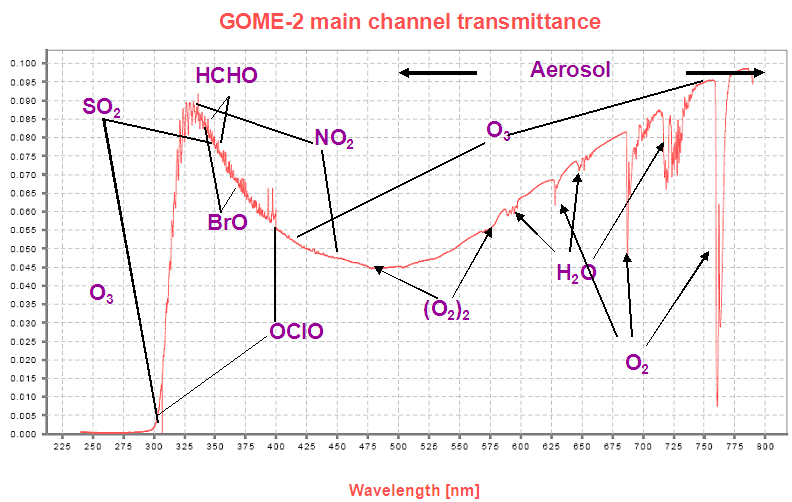
\includegraphics[width=\textwidth]{Figures/GOME_SPECTRUM.jpg}
      \caption{An example spectrum showing interferences used for species concentration measurements by GOME-2. Image by EUMETSAT and ESA (\cite{GOME2Image}.})
      \label{LR:HCHO:SatelliteDetection:fig_GOME_products}
    \end{figure}
    
    Satellites record near nadir (vertical) reflected spectra between around 250-700~nm split into spectral components at around $0.3$~nm in order to calculate trace gases including O$_3$, NO$_2$, and HCHO (eg: \cite{Leue2001}).
    Several public data servers are available which include products from satellites, including NASAs Earthdata portal (\url{https://earthdata.nasa.gov/}) and the Belgian Institute for Space Aeronomy (IASB-BIRA) Aeronomie site (\url{http://h2co.aeronomie.be/}).
    
    
    Instruments including MODIS on board the AQUA and TERRA satellites are able to determine aerosol optical depth (AOD), a measure of atmospheric scatter and absorbance. 
    An AOD of under 0.05 indicates a clear sky, while values of 1 or greater indicate increasingly hazy conditions.
    This is an important atmospheric property allowing us to track dust storms and pollution events as well as determine where measurements from other instruments may be compromised by high interference.
    Satellite measured AOD requires validation by more accurate ground based instruments like those of AERONET which uses more than 200 sun photometers scattered globally. 
    
    \subsubsection{OMI measurements}
    
      The OMI instrument on board AURA has been active since July 2005, it records spectra from 264-504~nm using an array of 60 detectors with mid-resolution (0.4-0.6~nm).
      This band of wavelengths allows measurments of trace gases including O$_3$, NO$_2$, SO$_2$, HCHO, and various other quantities like surface UV radiation.
      Recently \cite{Schenkeveld2017} analysed the performance over time of the instrument and found irradiance degradation of 3-8\%, changed radiances of 1-2\%, and a stable wavelength calibration within 0.005-0.020~nm.
      They also provide a very nice summary of the OMI instrument copied here in Fig. \ref{LR:HCHO:SatelliteDetection:fig_Shenkeveld_OMI_summary}, as it shows the instruments spectral, temporal, and spatial resolutions.
      These changes are measured excluding the row anomaly (RA) effect, which is relatively stable since 2011, although it is still growing and remains the most serious concern.
      An analysis of the row anomaly by \cite{Huang2017} state that OMI ozone columns remain suitable for scientific use, with recommendation for further evaluation.
      And analysis of OMI output by \cite{Schenkeveld2017} concludes that data is still of high quality and will deliver useful information for 5-10 more years, with radiances only changing by $1-2\%$ outside of RA impacted areas.
      The RA began in June 2007, with some cross-track rows seemingly blocked. The most likely cause is some instrument insulation partially obscuring the radiance port (\cite{Schenkeveld2017}).
      
      \begin{figure}
        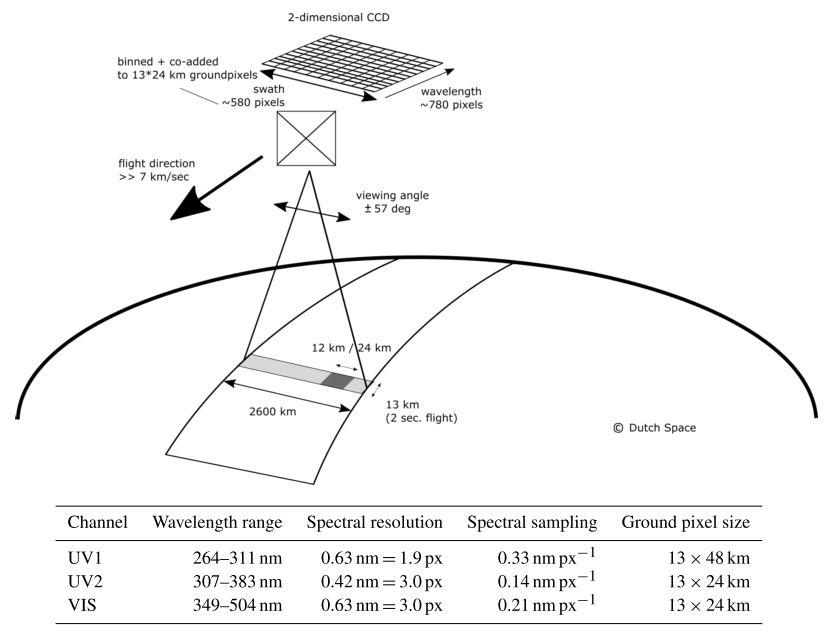
\includegraphics[width=\textwidth]{Figures/Shenkeveld_OMI_summary.png}
%        \caption{ %
%          Figure 1 and Table 1 from \cite{Schenkeveld2017}, with the following caption ``An impression of OMI flying over the Earth. The spectrum of a ground pixel is projected on the wavelength dimension of the charge-coupled device (CCD; the columns). The cross-track ground pixels are projected on the swath dimension of the CCD (the rows). The forward speed of 7~kms$^{-1}$ and an exposure time of 2~s lead to a ground pixel size of 13~km in the flight direction. The viewing angle of 114\degr leads to a swath width on the ground of 2600~km.''
%          The table shows the optical properties for OMIs three channels.}
        \label{LR:HCHO:SatelliteDetection:fig_Shenkeveld_OMI_summary}
      \end{figure}
      
      Soon even more HCHO data will be available in the form of geostationary satellite measurements (\cite{Kwon2017}).
      \cite{Kwon2017} examine simulated geostationary measurements against GEOS-Chem column simulations to determine the most important instrument sensitivities.
      Geostationary satellites can provide temporally rich measurements over an area, as they are not sweeping around the earth but fixed relative to one latitude and longitude.
    
    
    \subsubsection{DOAS}
      TODO: some of this is repeated in isoprene chapter satellite section.
      
      The DOAS technique uses solar radiation absorption spectra to measure trace gases through paths of light.
      The RTM used in DOAS techniques is based on Beer's law relating the attenuation of light to the properties of the medium it travels through.
      Beer's law states that $ T = I/I_0 = e^{-\tau} $ with T being transmittance, $\tau$ being optical depth, and I, I$_0$ being radiant flux received at instrument and emitted at source respectively.
      From $ \tau_i = \int \rho_i \beta_i ds $ we get:
      $$ I = I_0 \exp {\left( \Sigma_i \int \rho_i \beta_i ds \right) } $$
      Where i represents a chemical species index, $\rho$ is a species density(molecules per cm$^3$), $\beta$ is the scattering and absorption cross section area (cm$^2$), and the integral over ds represents integration over the path from light source to instrument.
      The forward RTM used for satellite data products also involves functions representing extinction from Mie and Rayleigh scattering, and the efficiency of these on intensities from the trace gas under inspection, as well as accounting for various atmospheric parameters which may or may not be estimated (e.g. albedo).
      
    \subsubsection{AMF}
      To convert the trace gas profile from a reflected solar radiance column (slanted along the light path) into a purely vertical column requires calculations of an air mass factor (AMF).
      In satellite data, the AMF is typically a scalar value for each horizontal grid point which will equal the ratio of the total vertical column density to the total slant column density.
      This value should also account for instrument sensitivities to various wavelengths at various altitudes, and is unique for each trace gas under consideration.
    
      An AMF characterises measurement sensitivity to a trace gas at various altitudes \cite[e.g.]{Palmer2001}.
      \cite{Lorente2017} show that AMF calculations can be the largest source of unertainty in satellite measurements.
      Another way of describing AMFs are as measures of how radiance at the top of the atmosphere (TOA) changes with trace gas optical depths at specific altitudes (\cite{Lorente2017}).
      Calculation of the AMF is important as it is multiplied against the estimated slant columns in order to give vertical column amounts.

      Related to the AMF is the averaging kernal (AK), which is used to handle instrument measurements which are sensitive to concentrations at different altitudes in the atmosphere.
      DOAS methods can be heavily influenced by the initial estimates of a trace gas profile (the apriori) which is often produced by modelling, so when comparing models of these trace gases to satellite measurements extra care needs to be taken to avoid introducing bias from differing apriori assumptions.
      One way to remove these apriori influences is through the satellites AK (or by using AMFs), which takes into account the vertical profile of the modelled trace gas and instrument sensitivity to the trace gas (\cite{Eskes2003, Palmer2001}).
      % TODO read and note this paper:
      \cite{Lamsal2014} recommends that when comparing satellite data to models, the AMF should first be recalculated using the model as an apriori.
      This is in order to remove any apriori bias between model and satellite columns.
    
    \subsubsection{Satellite uncertainties}
      %% grid size and averaging
      Satellite measurements of HCHO are relatively uncertain, however this can be improved by averaging over larger grid boxes or longer time scales.
      An example of this can be seen in \cite{Dufour2009}, where monthly averaging is used to decrease the measurements uncertainty.
      They examine HCHO in Europe, which is low; near the detection limit of satellite measurements.
      Taking monthly averages allows enough certainty that useful inversions can be determined to estimate the source emissions of HCHO.
      The finer nadir resolution of OMI (13 by 24~km${^2}$) compared to other satellites reduces cloud influence (\cite{Millet2006, Millet2008}). 
      Although the uncertainty in each pixel is $\sim 2 \times 10^{16}$, which is $5 \times$ higher than GOME, there are $\sim 100-200 \times $ as many measurements due to the smaller footprint and better temporal resolution of OMI, which allows a greater reduction of uncertainty with averaging (\cite{Chance2002,Millet2008}).
      
      %% SURFACE CONDITIONS AND CLOUDS
      In cloudy, hazy or polluted areas measurements are more difficult to analyse (\cite[e.g.][]{Palmer2003,Marais2014}).
      Recent work by \cite{Vasilkov2017} showed that updating how the surface reflectivity is incorporated into satellite measurements can change the retrievals by 50~\% in polluted areas.
      
      %% BACKGROUND MEASUREMENTS
      In satellite HCHO products, concentrations over the remote pacific ocean are sometimes used to analyse faulty instrument readings.
      This is due to the expected invariance of HCHO over this region.
      For instance GOME (an instrument which measures trace gases on board the ERS-2) corrects for an instrument artifact using modelled HCHO over the remote pacific (\cite{Shim2015}).
      OMI HCHO products use a similar technique to account for sensor plate drift and changing bromine sensitivity (\cite{Abad2015})
      
      
      %% EXAMPLES OF BIAS
      For many places the tropospheric column HCHO measured by satellite is biased low, \cite{Zhu2016} examine six available datasets and show a bias of 20 - 51\% over south east USA when compared against a campaign of aircraft observations (SEAC$^4$RS).
      \cite{DeSmedt2015} also found a low bias from 20 - 40\% when comparing OMI and GOME2 observations against ground based vertical profiles, and \cite{Barkley2013} determine OMI to be 37\% low compared with aircraft measurements over Guyana.
      These bias can be corrected by improving the assumed apriori HCHO profiles which are used to calculate the AMFs of the satellite columns.
      \cite{Millet2006} examine OMI HCHO columns over North America and determine overall uncertainty to be 40\%, with most of this coming from cloud interference.
      \cite{Millet2008} shows that there also exists some latitude based bias, as well as a systematic offset between the OMI and GOME instruments.
      This does not appear to be due to the different overpass times of the two instruments.
      
      %% UNCERTAINTY CALCULATIONS
      Uncertainty in the OMI satellite instrument is calculated by the Smithsonian Astrophysical Observatory (SAO) group using the uncertainty in backscattered radiation retrievals (\cite{Abad2015, Abad2016}).
      Another method of calculating the uncertainty is used by the Belgian Institute for Space Aeronomy (BIRA) group, who determine uncertainty from the standard deviation of HCHO over the remote pacific ocean \citep{DeSmedt2012, DeSmedt2015}.
      
      A full analysis of the AMF uncertainty in OMI measurements, as well as the structural uncertainty (between different systems of calculations applied to the same data) is performed by \cite{Lorente2017}.
      They determine the structural uncertainty using ensemble techniques on seven AMF calculation approaches used by different retrieval groups.
      They show that in scenarios where the gas is enhanced in the lower troposphere, AMF calculation is the largest uncertainty in satellite measurements.
      In polluted environments the structural uncertainty is estimated at 42~\%, or 31~\% over unpolluted environments.
      The importance of apriori and ancilliary data (such as surface albedo and cloud top height) is also shown, as it sharply affects the structural uncertainty.
      
      GOME suffers from similar uncertainties to OMI, as the same general method of DOAS remote measurements are performed.
      The uncertainty from slant column fitting has been calculated for GOME to be $4\times10^{15}$ molecules cm$^{-2}$ \citep{Chance2000, Millet2006}. 
      The conversion factor for slant to vertical columns (AMF) calculation also suffers from errors; primarily from surface albedo, HCHO vertical profile apriori, aerosol, and cloud influence \citep{Millet2006}. 
      AMF uncertainties for GOME are calculated to be $1$ to $1.3\times10^{15}$ molecules cm$^{-2}$ by \cite{Shim2005}.
    
    
  \subsection{Glyoxyl TODO: move somewhere fitting?}
  
    Another chemical retrievable from satellite observation is Glyoxyl, which can be used to further determine what sort of precursors to HCHO are being emitted \citep{Stavrakou2009, Miller2014, Miller2017}.
    TODO: go through 2014 paper and see if it's easy to retrieve, then email Dr. Chris Miller.
    For example \cite{Cao2018_discuss} recently used Glyoxyl measurements to improve understanding of biogenic and anthropogenic NMVOC emissions over China.
    This involved using a method pioneered by \cite{Stavrakou2009} TODO: get this cite and check method out.
   
    Glyoxyl (CHOCHO) is important to us as it shares many properties with HCHO, and may provide additional information in determining isoprene emissions.
    Glyoxyl is another product of VOC oxidation in the atmosphere, with isoprene being the main source globally.
    Under high NO$_X$ conditions, glyoxyl forms rapidly, similarly to HCHO.
    However, glyoxyl also forms in low NO$_X$ environments both slowly (through isoprene epoxydiols), and rapidly (through di-hydroperoxide dicarbonyl compound photolysation \citep{Crounse2013}.
    This process is similar to the proposed mechanisms for hydroperoxyaldehydes by \cite{Peeters2014} and carbonyl nitrates \citep{Muller2014}.
    Aromatics which are largely anthropogenic form glyoxyl quickly, while HCHO is produced slower, allowing determination of anthropogenic sources \citep{Cao2018_discuss}.
    
    HCHO has been used to estimate isoprene emissions (some examples in Section \ref{LR:HCHO:SatelliteInversion}) but many uncertainties exist.
    One of these uncertainties is the yield of HCHO from isoprene, especially in low NO$_X$ environments.
    Glyoxyl could prove complementary to HCHO in constraining isoprene emissions (TODO: Read and cite Vrekoussis2009,2010, Chan Miller 2014, Alvarado 2014) \citep{Miller2017}.
    Recently \cite{Miller2017} updated GEOS-Chem to include the prompt formation of glyoxyl and compared this with satellite and airplane measurements over the USA.
    Glyoxyl is formed by isoprene oxidation rapidly in low NO$_X$ conditions, unlike HCHO.
    With coming geostationary satellites, which provide greater time resolved measurements of HCHO and CHOCHO, this mechanism could be used to clearly show when low NO$_X$ isoprene chemistry is being undertaken \citep{Miller2017}.
    
\section{Models}
  \label{LR:Models}
  \subsection{How can models help}
    
    Models can fill the gaps (both spatial and temporal) in measurement records, and are used to predict/avoid/mitigate hazardous scenarios.
    They are used ideally to steer us away from unsustainable pollution and help complete our understanding of the world from small to large scales.
    They can be used to increase measurement accuracy (for instance in satellite measurements) and determine where we lack information, while also checking the performance of new instruments.
    Precisely representing various chemicals and reactions in the atmosphere allows efficient mitigation of pollution, since we can compare scenarios against one another.
    Currently, improved isoprene understanding is critical for effective air quality measuring \citep{Marvin2017}.
    
    Chemical Transport Models (CTMs) simulate production, loss, and transport of chemical species.
    This is generally calculated using one or both of the Eulerian (box) or Lagrangian (puff) frames of reference.
    CTMs normally solve the continuity equations simultaneously with chemical production and loss for chemicals under inspection. 
    The continuity equations describe transport of a conserved quantity such as mass, which, solved together with production and loss of a chemical can provide detailed simulations of natural processes.
    Models provide a simulation of chemical densities and transport over time as a model runs.
    The general continuity equation links a quantity of a substance (q) to the field in which it flows and can be described by the formula:
    \begin{eqnarray*}
      \frac{\partial \rho}{\partial t} + \nabla \cdot j &=& \sigma 
    \end{eqnarray*}
    where $\rho$ is density of q in the field, t is time, $\nabla$ is divergence, j is the flux (q per unit area per unit time entering or leaving the field), and $\sigma$ is the generation or loss of q per unit volume per unit time.
    
    
    The type of model best suited to modelling the entire earth uses the Eulerian frame of reference, where the atmosphere is broken up into 3-D boxes with densities and transport calculated and stored for sequential steps in time at each location.
    The mass balance equation must be satisfied in any realistic long term box model and is as follows: 
    \begin{align*}
      \frac{dm}{dt} &=& \sum{sources}-\sum{sinks} \\
      &=& F_{in} + E + P - F_{out} - L - D 
    \end{align*}
    where m is mass of a chemical, E and D are emission and deposition, P and L are production and loss, and F is chemical transport in and out, as shown in figure \ref{LR:Models:fig_boxmodel}.
    Many chemical species interact with each other through production and loss. 
    Any large chemical model will solve this mass balance equation over highly coupled arrays of partial differential equations which can be complex and time consuming.
    
    \begin{figure}
      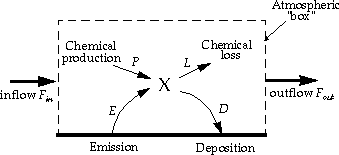
\includegraphics{Figures/boxmodel.png}
      \caption{ %
        Standard box model parameters, image taken from \cite{Jacob_1999_book}. }
      \label{LR:Models:fig_boxmodel}
    \end{figure}
    
    In many CTMs the isoprene emissions are calculated seperately using MEGAN, and then used as boundary conditions (EG: \cite{Guenther2006}). 
    This can speed up calculations as the transport and concentrations can be simulated in various conditions without recalculating the emissions.
    Trace gases with short lifetimes and complex chemistry such as isoprene are often hard to measure which makes verifying model estimates difficult.
    Contemporary models generally use mathematical differential solving tools of various complexity to solve chemical equations and reaction rates (often called chemical mechanisms) in order to predict an environments evolution over time.
    Different solvers may be slower or faster and more suited to particular situations based on the stability of the equations and systems involved, and chemical mechanisms may vary in how many reactions and chemicals are listed and grouped together.
    For example: Since [O] $<<$ [O$_3$] the chemical family O$_X$ (  O$_X \equiv $ O $+$ O$_3$ ) can be used to simplify chemistry simulations and approximate O$_3$ concentrations \citep[][Chapter 3]{BrasseurJacob2017}.
    \cite{Zhang2012} examine the outputs from a regional model (WRF/Chem) using three different chemical mechanisms, and they show that particulate matter prediction is sensitive to the choice of chemical mechanism. 
    
  \subsection{Relevant model frameworks}
  \label{LR:Models:frames}
    
    % Outline of ACM
    Atmospheric chemistry models (ACMs) require various inputs and can be sensitive to ozone and oxidative parameterisations. 
    TODO: read more Christian 2017,
    TODO: put some more generic ACM info here.
    
    \subsubsection{Box models} 
    \label{LR:Models:frames:box}
    % for example CAABA/MECCA
      A box model involves modelling chemistry in a singular set of conditions without transport or any spatial gradients.
      One box model used in this thesis is called CAABA/MECCA, and is described here as an example.
      
      CAABA (Chemistry As A Boxmodel Application) estimates the chemical concentrations accounting for J-values (JVAL), simplified and parameterised photolysis (SAPPHO) and simplified emission and depositions (SEMIDEP).
      CAABA runs in a single scenario (or box) with given emissions, depositions, and initial concentrations, allowing the examination of chemistry in a very specific environment to be modelled with high temporal resolution.
      This has been used with an atmospheric chemistry model MECCA (Module Efficiently Calculating the Chemistry of the Atmosphere) which implements tropospheric and stratospheric chemistry for both the gas and the aqueous phases \citep{Sander2005}.
      MECCA chemical mechanisms include basic O$_3$, CH$_4$, NO$_X$, and HO$_X$ chemistry, as well as non methane hydrocarbon (NMHC) chemistry, considering gas phase, aqueus phase, and heterogenous reactions. \citep{Sander2005}
      For the numerical integration, MECCA uses the KPP software (\cite{SanduSander2006}), which takes chemical reactions and their rate coefficients and codes integral solutions to the system.
      The combination of the CAABA box model with MECCA module is called CAABA/MECCA and is currently at version 3.
      CAABA/MECCA been implemented for various calculations including ozone chemistry throughout the atmosphere in \cite{Zanis2014}.
  
      MECCA could also be used as the chemistry mechanism for a more complex, 3-dimensional model (\cite[e.g.][]{Jockel2006}).
      The connection is established via the MESSy interface (\url{http://www.messy-interface.org}) developed by \cite{Jockel2005} as part of an effort to simplify the framework for modelling the atmospheres at various scales.
      The user manual is available online at \url{http://www.rolf-sander.net/messy/mecca/caaba_mecca_manual.pdf}.
  
      By allowing for interactions between boxes this concept can be extended to multiple-box models.
      These are simply multiple instances of single boxes with the addition of transport between them, which generally requires a meteorological model to provide winds, and other transport mechanisms.
      
    \subsubsection{Chemical transport} %% eg. GEOS-Chem
      GEOS-Chem is an example of this, with many boxes covering the globe, each with chemistry and dynamic meteorological conditions.
      The transport between boxes also needs to be taken into account when simulating concentrations.
      Additionally the different meteorological conditions such as wind and air pressure need to be handled within each box.      
      GEOS-Chem has a meteorological model coupled to a chemical model, which simulates the world in a three dimensional grid of connected boxes.
      
      GEOS-Chem is a well supported global, Eulerian CTM with a state of the science chemical mechanism, with transport driven by meteorological input from the Goddard Earth Observing System (GEOS) of the NASA Global Modeling and Assimilation Office (GMAO).
      GEOS-Chem simulates more than 100 chemical species from the earth's surface up to the edge of space (0.01~hPa) and can be used in combination with remote and in-situ sensing data to give a verifiable estimate of atmospheric gases and aerosols.
      It was developed, and is maintained, by Harvard University staff as well as users and researchers worldwide.
      Several driving meteorological fields exist with different resolutions, the finest at 0.25 by 0.3125$^\circ$ horizontally at 5 minute time steps with 72 vertical levels.
      
      Global CTMs are often run using one or several emission models (or the output from them) to determine boundary conditions for many gridboxes.
      TODO: is this the case? Doesn't GEOS-Chem have coupled chemistry and meteorology? Check the wiki.
      GEOS-Chem has boundary conditions based on several meteorological and emissions inventories, the following are the versions of theses used by GEOS-Chem v 10.01. 
      Meteorological fields can be driven by NASA's GEOS-5 data (0.5$^{\circ}$ x 0.666$^{\circ}$) \citep{Chen2009}, which exists up to 2013, or GEOS-FP data (0.25$^{\circ}$ x 0.3125$^{\circ}$).
      Fire emissions come from the GFED4 product \citep{Giglio2013}. 
      Anthropogenic VOC emissions come from the EDGAR inventory, while biogenic VOC emissions are coupled to the MEGAN model TODO:cites.
      The estimated biogenic VOC emissions are important for accurately simulating chemistry within models, as discussed in Sections \ref{LR:O3andAQ:BiogenicOzonePrecursors} and \ref{LR:Models:Unc}.
      
      The Model of Emissions of Gases and Aerosols in Nature (MEGAN) is one of the more commonly used natural emission models \citep{Monks2015}. (TODO: more cites which say this/use MEGAN)
    
    \subsubsection{Land based emissions} %% EG MEGAN
      % TODO: Overview of land based emissions modelling?
      
      MEGAN is a global model with resolution of around 1~km, and is used to generate the BVOC emissions used in various global chemistry models such as GEOS-Chem.
      MEGAN uses leaf area index, global meteorological data, and plant functional types (PFTs) to simulate terrestrial isoprene emissions.
      The model includes global measurements of leaf area index, plant functional type, and photosynthetic photon flux density, from remote sensing databases \citep{Kefauver2014}.
      The various PFTs are used to generate emission factors which represent quantities of a compound released to the atmosphere through an associated activity.
      For example, an emission factor for isoprene within a forest would include the requirement of sunshine and suitable temperature.
      The schematic for MEGAN, taken from \citet{Megan_Website}, is shown in figure \ref{LR:models:frames:fig_megan_schematic}
      
      \begin{figure}[!htbp]
        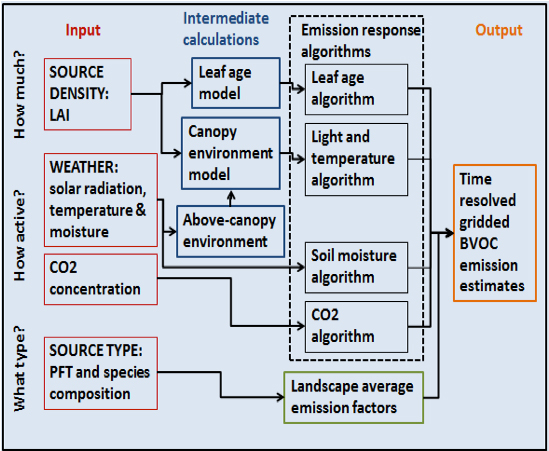
\includegraphics[width=\textwidth]{Figures/MEGANmodel_img.jpg}
        \caption{MEGAN schematic, copied from \citet{Megan_Website}}
        \label{LR:models:frames:fig_megan_schematic}
      \end{figure}
      
      MEGAN ``is a modelling framework for estimating fluxes of biogenic compounds between terrestrial ecosystems and the atmosphere to account for the major known processes controlling biogenic emissions.'' \citep{Guenther2012}.
      It allows parameterisation of various BVOC emissions, with descriptions given in \cite{Guenther2012}.
      Instructions to run version 2.1 are available at \url{http://lar.wsu.edu/megan/docs/MEGAN2.1_User_GuideWSU.pdf}, and a version using the Community Land Model (CLM) is available at \url{http://www.cesm.ucar.edu}.
      It uses meteorological fields from the Weather Research and Forecasting (WRF) modelling system.
      Version 2.1 (updated from 2.0 \citep{Guenther2006}) includes 147 species, in 19 BVOC classes, which can be lumped together to provide appropriate output for mechanisms in various chemical models.
      
      MEGAN was developed as a replacement for two earlier canopy-environment emission models (BIES and GEIA), and initially included a simple canopy radiative transfer model, which parameterised sun-lit and shaded conditions through a canopy.
      Early models didn't account for abiotic stresses, such as drought, prior rainfall and development processes, although these influenced species specific emissions by more than an order of magnitude \citep{Niinemets1999}.
      Isoprene emissions were based on temperature, leaf area, and light, but have since been updated to include leaf age activity \citep{Guenther2000}, and a leaf energy balance model \citep{Guenther2006} in MEGANv2.0.
      This update included a parameter for soil moisture, to account for drought conditions, however this parameter is currently (as of version 2.1) not applied to isoprene \citep{Sindelarova2014}.
      Soil moisture effects on isoprene emission are very important, and can drastically affect estimates.
      
      MEGAN has recently been analysed using 30 years of meteorological reanalysis information by \cite{Sindelarova2014}.
      They estimate emissions of Biogenic VOCs (BVOCs) to be 760~Tg(C)yr$^{-1}$, 70\% (532~Tg(C)yr$^{-1}$) of which is isoprene.
      This is similar to isoprene emission estimates from MEGAN itself, of 400-600~Tg(C)yr$^{-1}$ \citep{Guenther2006}.
      MEGAN emissions estimates are termed bottom-up, as opposed to top-down which are derived from satellite measurements of the products of various VOCs.
      Using GOME satellite HCHO and a Beyesian inversion technique to derive isoprene emissions, \cite{Shim2005} estimated global isoprene emissions to be $\sim566$~TgC yr$^{-1}$. 
      This estimate is greater than initially thought and leads to decreased ($\sim10\%$) simulated OH concentrations to 9.5e5 molec cm$^{-3}$.
      
      Improvements to emissions models require improved understanding of regions and their behaviour.
      Inaccuracies can arise due to lack of data, such as the large and sparsely measured Australian outback.
      MEGAN has been shown to overpredict isoprene and underpredict monoterpene emissions in southeast Australia, with peaks and troughs captured but not at the right magnitude (\cite{Emmerson2016}).
      MEGAN output in Australia is adversely affected by poor emission factor estimation. 
      An example can be seen in \citet{Muller2008} where MEGAN overestimates isoprene in northern Australia.
      Underestimates of monoterpenes may be due simply to underestimated emission rates for many Eucalypt species \citep{Winters2009}.
      

    \subsubsection{Radiative transfer} %% EG LIDORT
      %TODO: Lidort example?
      TODO: Lidort example?
    
  \subsection{Factors affecting isoprene emissions estimates}

      \cite{Marais2014} examine factors affecting isoprene emissions, showing how emissions are sensitive to various environmental factors.
      Their work used MEGAN \citep{Guenther1995} and GEOS-Chem to look at how these factors affect surface ozone and particulate matter in Africa.
      One of the important uncertainties seen in MEGAN within this work is the isoprene emissions due to plant type.
      Canopy level isoprene measurements are made using relaxed eddy accumulation (REA) at several sites in Africa.
      One plant type near a measurement site emits more than other species and it's actual distribution on a larger scale is completely unknown - leading to possible overestimations in MEGAN.
      Current emissions estimates require more validation against observations, and recently a comparison of two major VOC models (MEGAN and ORCHIDEE) was undertaken by \cite{Messina2016} reiterating this requirement.
      In their work they examine model sensitivities and show that the important parameters are leaf area index (LAI), emission factors (EF), plant functional type (PFT), and light density fraction (LDF).
      There is high uncertainty in LAI and EF, which require more or improved measurements at the global scale.
      LDF paramterisation needs improvement and these models require more PFTs.
      Global emissions inventories like MEGAN suffer from large extrapolations which introduce uncertainties \citep{Miller2014}.

      \cite{Emmerson2016} analyse EF sensitivity of a high resolution model of atmospheric chemistry over southeast Australia, comparing isoprene and monoterpene emissions against 4 separate campaigns.
      They show that the effect on total emissions is roughly linear and that no blanket EF changes are appropriate for all regions/seasons.
      They also mention that Australian eucalypt emissions are based on samples from young trees, which may emit more isoprene than older trees.
      
      \cite{Stavrakou2014} examined modelled Asian emissions and altered model parameters for temperature, plant type emission factors, incoming solar radiation (insolation) intensity, land use changes, and palm tree forest expansion.
      Changes were constrained by a network of radiation measurements and some experiments with south east Asian forest emissions - and led to reduction in isoprene emissions by a factor of two over the region.
      The Asian region is also shown to have a strong correlation with the Oceanic Niño Index (ONI), with positive anomalies associated with El Niño.
      In the last 20 years anthropogenic emissions of VOCs have been increasing while biogenic VOC emissions have decreased due to rapid economic growth and lower annual temperatures \citep{Stavrakou2014, Kwon2017}.
      
      %Temperature has a strong exponential relationship with isoprene emissions, and can be readily seen in comparisons to a major isoprene product HCHO. 
  
  % TODO: Reading up to here
  \subsection{Uncertainties}
    \label{LR:Models:Unc}
    Here I will attempt to list and partially explain the major uncertainties models have in relation to  VOCs, SOAs, and ozone. 
    TODO: Is this a good idea or should I put any pertinent uncertainties with the associated work/descriptions?
    
    \subsubsection{Emissions Inventories}
      % Emissions Inventories 
      Using different emissions inventories in an ACM can have large impacts on the simulation.
      Natural (biogenic or pyrogenic) and human driven (anthropogenic) emissions often drive a large fraction of atmospheric oxidation and radical chemistry, especially in the continental boundary layer.
      \cite{Zeng2015} examine the affects on CO and HCHO when running simulations with two different inventories.
      TODO: find where I took notes about Zeng2015 and put them here.
    
    %% GEOS-Chem resolution uncertainties
    \subsubsection{Resolution}
      \label{LR:Models:Unc:Resolution}
      GEOS-Chem simulations are somewhat sensitive to the resolution at which you run.
      For example: \cite{Wild2006} show that reduced resolution increases OH concentrations and ozone production rates.
      \cite{Christian2017} find small changes in OH ($<10$\%) in OH, HO$_2$ and ozone concentrations local to the north american arctic, when changing from 4 by 5 to 2 by 2.5\degr resolution, however they continue at lower resolution to save computational time.
      
      For many global scale analyses, errors from resolution are less important than those from chemistry, meteorology, and emissions (\cite{Christian2017}).
      
    
    % Transport uncertainties?
    \subsubsection{Transport}
      \label{LR:Models:Unc:Transport}
      TODO: Literature showing transport uncertainties or lack thereof     
      %TODO: examples of transport uncertainties
    
    \subsubsection{Chemistry mechanisms}
      \label{LR:Models:Unc:Chemistry}
      %% GEOS-Chem Ozone uncertainties 
      There is still much work to be done in models to correctly simulate the various precursors to HCHO.
      Often HCHO is used as a way of checking if these precursors are correctly modelled since HCHO measurements are more readily available (for instance from satellites).
      GEOS-Chem has recently been analysed for sensitivity for ozone along with oxidants (OH and HO$_2$) \citep{Christian2017}.
      \cite{Christian2017} found that GEOS-Chem ozone was most sensitive to NO$_2$ photolysis, the $NO_2 + OH$ reaction rate, and various emissions.
      They used GEOS-Chem v9-02, with $4^{\circ} \times 5^{\circ}$ resolution, and while the low resolution adds errors in OH concentrations and O$_3$ production rates, the errors from chemistry, meteorology, and emissions are much larger.

      \cite{Marvin2017} suggest that isoprene mechanisms in several contemporary models (including GEOS-Chem) are inadequate. 
      They show that for a specific measurement campaign, the HCHO concentrations are underestimated in a way that can not be easily fixed through rate constant changes.
      Recently \cite{Marvin2017} compared five global ACMs isoprene mechanisms by evaluating simulated HCHO mixing ratios compared to in situ measurements from the Southeast Nexus (SENEX) aircraft campaign (in southeastern USA).
      They compared five models (GEOS-Chem, CB05, CB6r2, MCMv3.2, and MCMv3.3.1) and found all of them underestimated the HCHO concentrations (by $15 - 30\%$).
    
    \subsubsection{Clouds}
      \label{LR:Models:Unc:Clouds}
      One of the major uncertainties in chemical, climate, radiation, and weather models is cloud formation and dynamics.
      Clouds are remarkably complex at a much finer scale than can be accurately modelled by global chemistry models (with current processing power).
      Globally over half (50-60\%) of the world is covered by clouds, with $\sim10\%$ of them being rain-clouds \citep{Kanakidou2005}.
      Wet scavenging performed in clouds not only depends on large scale cloud processes, but also on the microphysics of aerosols being scavenged, differing between aerosol sizes and hygroscopic properties.
      
    \subsubsection{Soil Moisture}
      \label{LR:Models:Unc:SoilMoisture}
      Australia has a unique climate, along with soil moisture, clay content and other important properties which affect VOC emissions.
      These properties are poorly understood in Australia due to the continents size and the relative sparsity of population centres, which make many areas very difficult or expensive to reach.
      Soil moisture plays an important role in VOC emissions, as trees under stress may stop emitting various chemicals. 
      This is especially true for Australia due to frequent droughts and wildfires.
      The argument for improved understanding of land surface properties, specifically soil moisture, is an old one\citep{Mintz1982, Rowntree1983, Chen2001}. 
      \cite{Rowntree1983} show how quickly soil moisture anomalies affect rainfall and other weather systems, while \cite{Chen2001} specifically show how important fine scale soil moisture information is when modelling land surface heat flux, and energy balances.
      Modelled emissions are sensitive to soil moisture, especially near the soil moisture threshold (or wilting point), below which trees stop emitting isoprene and other VOCs completely as they can no longer draw water \citep{Bauwens2016}.
      MEGAN accounts for soil moisture by applying it as an emission factor (EF) which scales the emission rate of various species.
      \cite{Sindelarova2014} show reductions in modelled Australian isoprene emissions of 50\% when incorporating soil moisture in MEGAN estimates. 
      
      Droughts affects can be difficult to measure, as it is a multi-scale problem which affects various aspects of the land-air interface including plant emissions and dry deposition (\cite{Wang2017}).
      The Standardised Precipitation Evapotranspiration Index (SPEI) is a measure of drought using TODO \cite{SPEI_website}.
      This product covers 1901 - 2011, and uses the average over that period as the background, in order to compare drought stressed regions against those with sufficient or excess water \cite{SPEI_website}.
      
